\section{系统模型}
\subsection{场景建模}
考虑边长为$L$的正方形区域，部署$N$架具备通信与计算能力的无人机，为$K$个地面用户提供服务。无人机集合与用户集合分别记为$\mathcal N=\{1,\ldots,N\}$和$\mathcal K=\{1,\ldots,K\}$，下文用$n,i,j$索引无人机，用$k$索引用户。用户$k$的固定源无人机记为$a_k\in\mathcal N$，关联用户集合为$\mathcal K_n=\{k:a_k=n\}$。固定源关联表示用户移动后仍向同一源无人机上传，源节点可通过协作转移计算工作；它不等于用户始终停留在原区域，也不包含动态切换关联机制。

图\ref{fig:system}给出了网络组成。无人机具有相同高度$h$，用户$k$与无人机$n$在物理步$m$的水平位置分别为$\vct u_k[m]\in[0,L]^2$和$\vct q_n[m]\in[0,L]^2$，坐标单位均为m。用户采用参考点群组移动（reference point group mobility，RPGM）方式运动：同一群组共享缓慢移动的参考点，各用户叠加具有记忆性的局部速度，并通过回复项保持群组联系。参考点与局部运动均随时间更新，位置越界时执行边界修正。因此，空间热点既随用户群移动，也会因业务强度切换而改变，两者不是同一个随机过程。

\begin{figure*}[t]
\centering
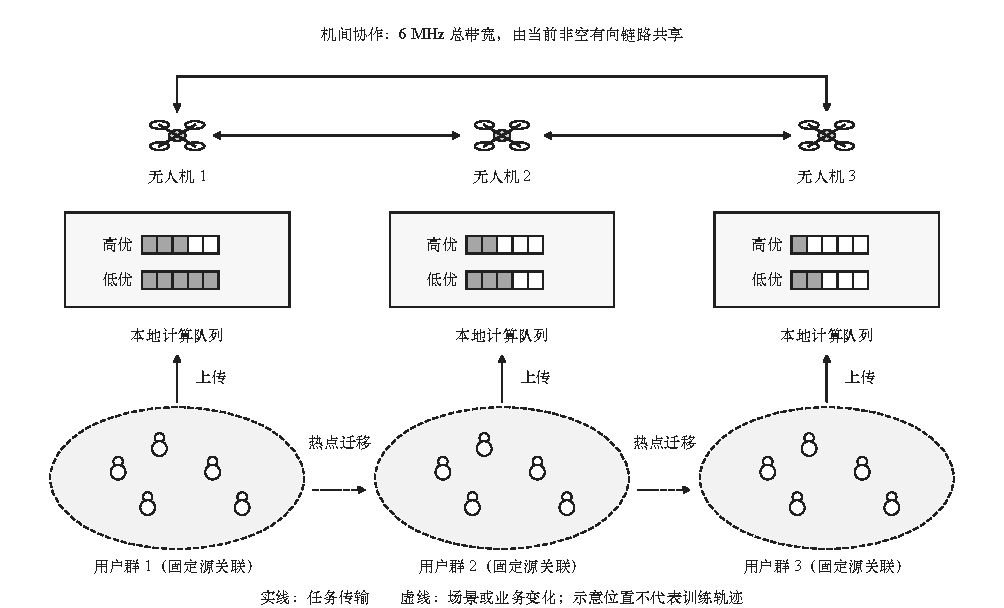
\includegraphics[width=\textwidth]{figures/fig1_system.pdf}
\caption{多无人机协同计算场景：固定源关联、分优先级计算及共享机间传输}
\label{fig:system}
\end{figure*}

系统包含大周期、资源帧与物理步三个时间单位，长度分别为$T_{\mathrm L}$、$\Delta$和$\delta$，均以s计。大周期编号为$t$，全局资源帧编号为$s$，全局物理步编号为$m$。一个资源帧包含$F=\Delta/\delta$个物理步，一个大周期包含$J=T_{\mathrm L}/\Delta$个资源帧，其中前$J_{\mathrm D}=T_{\mathrm D}/\Delta$帧用于部署，$T_{\mathrm D}$为部署时长。本文采用$T_{\mathrm L}=10$ s、$T_{\mathrm D}=1$ s、$\Delta=0.5$ s和$\delta=0.1$ s，即$F=5$、$J=20$、$J_{\mathrm D}=2$。

在大周期起点选择部署位置，完成移动后的位置在剩余服务期保持不变。路由仅在服务帧起点更新，并在帧内保持。令$\chi[m]\in\{0,1\}$表示服务开关，部署物理步取0，服务物理步取1。部署期间用户继续移动、任务继续产生，上传、机间传输与计算暂停。这样，部署收益与服务中断损失均进入同一任务演化过程，不通过额外的人工移动惩罚代替暂停时间。

任务优先级集合为$\mathcal P=\{\mathrm H,\mathrm L\}$，分别表示高、低优先级，用$p$索引。用户$k$在资源帧$s$产生的$p$类任务数为$A_{k,p}[s]$，采用条件泊松到达模型：
\begin{equation}
 A_{k,p}[s]\sim\operatorname{Poisson}(\lambda_{k,p}[s]\Delta).
 \label{eq:arrival}
\end{equation}
其中，$\lambda_{k,p}[s]$为当前到达强度，单位为task/s；给定当前业务阶段后，不同用户和类别分别采样。用户类型决定$p$类单任务数据量$b_{k,p}$，单位为Mbit。源节点$n$的期望输入负载为
\begin{equation}
 \ell_n[s]=\sum_{k\in\mathcal K_n}\sum_{p\in\mathcal P}
 \lambda_{k,p}[s]b_{k,p}.
 \label{eq:load}
\end{equation}
$\ell_n[s]$的单位为Mbit/s。每个业务阶段统一缩放同一源区域内的到达强度，使其满足设定负载，保留不同设备和优先级的相对业务差异。阶段切换只改变之后的到达，不清空已存在任务。控制器可获取当前负载配置和已观察的阶段年龄，不获取下一次切换的预先采样时刻。

任务记录用$\nu$索引，其出生时刻、数据量、优先级和源节点分别记为$\tau_\nu^{\mathrm b}$、$B_\nu$、$p_\nu$和$i_\nu$；出生时刻单位为s，数据量单位为Mbit。完整上传后的父任务才允许拆分，拆分之后不重新选择源节点，也不因下一帧路由变化而迁移已经分配的分片。回传结果的数据量、回传时间与控制信令开销暂不计入服务模型，故所定义的完成时刻为计算结果在计算节点可用的时刻。

\subsection{通信模型}
用户至无人机（user-to-UAV，U2G）与无人机间（UAV-to-UAV，U2U）传输采用正交资源，忽略不同正交链路间的干扰。设$\beta_0$为参考距离1 m处的功率增益参数，$\sigma^2$为接收机等效噪声功率，单位为W。用户上行发射功率为$P_{\mathrm G}$，全部用户共享的上行带宽为$B_{\mathrm G}$，分别以W和Hz计。上行带宽按全部$K$个用户等分，不随活跃用户数重新分配。于是
\begin{equation}
 R_k^{\mathrm G}[m]=\frac{B_{\mathrm G}}{K}
 \log_2\!\left(1+
 \frac{P_{\mathrm G}\beta_0}
 {\sigma^2(\|\vct u_k[m]-\vct q_{a_k}[m]\|_2^2+h^2)}
 \right).
 \label{eq:u2g}
\end{equation}
其中，$R_k^{\mathrm G}[m]$为用户$k$的上行速率，单位为bit/s。式\eqref{eq:u2g}采用自由空间距离衰减和固定等效噪声参数；本文不额外引入未建模的随机遮挡、快衰落或随带宽变化的噪声谱密度模型。

令$Q_{ij,p}^{\mathrm T}[m]$表示从$i$转发至$j$的$p$类队列在物理步起点的剩余待传数据量，单位为Mbit。物理步内的新分片先加入对应队列，再判定活跃链路。以$\widetilde Q_{ij,p}^{\mathrm T}[m]$表示加入新分片后的待传量，活跃链路集合为
\begin{equation}
 \mathcal A[m]=\left\{(i,j):i\ne j,\ 
 \sum_p\widetilde Q_{ij,p}^{\mathrm T}[m]>0\right\}.
 \label{eq:active}
\end{equation}
令$B_{\mathrm U}$为全部有向机间链路共享的总带宽，单位为Hz。当$\mathcal A[m]$非空时，链路$(i,j)$获得带宽
\begin{equation}
 B_{ij}[m]=
 \begin{cases}
 B_{\mathrm U}/|\mathcal A[m]|,&(i,j)\in\mathcal A[m],\\
 0,&\text{其他}.
 \end{cases}
 \label{eq:bandwidth}
\end{equation}
当集合为空时，全部机间带宽分配为0。链路$(i,j)$和$(j,i)$分别计数，而高、低优先级共用同一有向链路，不因存在两个优先级而重复计数。

机间发射功率记为$P_{\mathrm U}$，机间谱效率$\eta_{ij}[m]$和速率$R_{ij}^{\mathrm U}[m]$为
\begin{equation}
 \begin{aligned}
 \eta_{ij}[m]&=\log_2\!\left(1+
 \frac{P_{\mathrm U}\beta_0}
 {\sigma^2\|\vct q_i[m]-\vct q_j[m]\|_2^2}\right),\\
 R_{ij}^{\mathrm U}[m]&=B_{ij}[m]\eta_{ij}[m],\quad i\ne j.
 \end{aligned}
 \label{eq:u2u}
\end{equation}
其中，$\eta_{ij}[m]$无量纲，$R_{ij}^{\mathrm U}[m]$以bit/s计；对角项均设为0。安全间距约束避免两架无人机重合。总带宽共享使链路服务能力与全部转发队列有关，不能将$B_{\mathrm U}$直接代入每一条链路并假定各链路同时独占总带宽。

令$U_{k,p}[m]$为用户端$p$类剩余上传量，单位为Mbit；$A^{\mathrm G}_{k,p}[m]$为本物理步新进入上传缓冲的数据量，仅在任务到达时非零；$S^{\mathrm G}_{k,p}[m]$为实际上传量。其更新为
\begin{equation}
 U_{k,p}[m+1]=U_{k,p}[m]+A^{\mathrm G}_{k,p}[m]
 -S^{\mathrm G}_{k,p}[m].
 \label{eq:uploadqueue}
\end{equation}
用户上行服务满足
\begin{equation}
 \sum_p S^{\mathrm G}_{k,p}[m]
 \le \chi[m]R_k^{\mathrm G}[m]\delta/10^6.
 \label{eq:uploadcap}
\end{equation}
系数$10^6$用于bit到Mbit的换算；实际服务同时受剩余数据量限制，高优任务先获得服务。一个父任务的数据可跨多个物理步上传，完整上传只形成待路由任务，不等于已经完成计算。

令$S^{\mathrm T}_{ij,p}[m]$为物理步内实际机间传输量，同样以Mbit计，则
\begin{equation}
 \sum_pS^{\mathrm T}_{ij,p}[m]\le
 \chi[m]R_{ij}^{\mathrm U}[m]\delta/10^6.
 \label{eq:txcap}
\end{equation}
每条链路先服务高优队列，再将剩余传输容量用于低优队列，同类任务按队列顺序处理。此处的“高优先”是服务顺序，不构成高优任务必然满足某个确定时限的保证。

\subsection{计算与任务完成模型}
图\ref{fig:taskflow}展示了父任务处理链。对源节点$i$的$p$类新待路由任务，资源帧$s$采用比例$\rho_{ij,p}[s]$分配给目的节点$j$，其中$\rho_{ij,p}[s]$为无量纲标量，满足
\begin{equation}
 \rho_{ij,p}[s]\ge0,\qquad
 \sum_{j\in\mathcal N}\rho_{ij,p}[s]=1.
 \label{eq:simplexconstraint}
\end{equation}
对角比例表示源节点本地计算，非对角比例表示一次机间转发后在目的节点计算。两类路由矩阵共同记为$\vct\rho[s]\in\R^{2N^2}$，按优先级、源、目的顺序展平。允许任意一个非负比例为0，不强制每项任务都经过多台无人机。

\begin{figure*}[t]
\centering
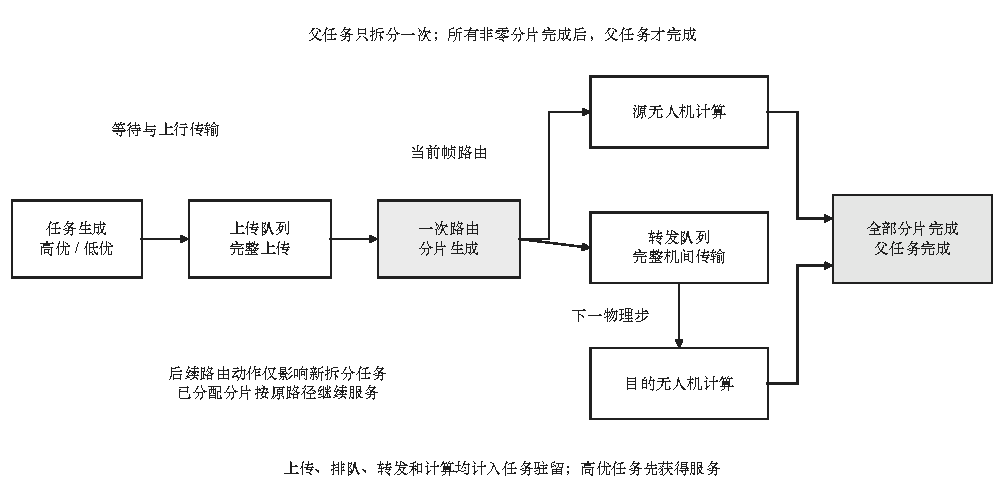
\includegraphics[width=\textwidth]{figures/fig2_taskflow.pdf}
\caption{父任务处理路径：完整上传后一次拆分，以所有非零分片完成作为父任务完成条件}
\label{fig:taskflow}
\end{figure*}

令$\mathcal V_{i,p}[m]$为在物理步$m$实际进行拆分的父任务集合。这些任务在之前的物理步已经完整上传，尚未形成计算分片。设$s(m)$为包含物理步$m$的资源帧，则新加入$(i,j,p)$路径的数据量为
\begin{equation}
 D_{ij,p}[m]=\sum_{\nu\in\mathcal V_{i,p}[m]}
 B_\nu\rho_{ij,p}[s(m)].
 \label{eq:split}
\end{equation}
$D_{ij,p}[m]$以Mbit计。在物理步内，先处理已有待路由任务，再推进用户上行，因此本步刚完成上传的任务在下一物理步拆分。该一物理步的处理先后关系不能与“资源帧起点更新一次路由”混淆。

令$Q_{n,p}^{\mathrm C}[m]$为节点$n$在步起点已完整到达、尚未完成计算的$p$类工作量，单位为Mbit。新本地分片可在本步参与计算，可用计算工作量为$\widetilde Q_{n,p}^{\mathrm C}[m]=Q_{n,p}^{\mathrm C}[m]+D_{nn,p}[m]$。设$C$为中央处理器（central processing unit，CPU）处理1 bit所需的周期数，单位为cycle/bit；$F_n^{\max}$为节点最大CPU频率，单位为cycle/s。为在一个物理步内清空该类工作量，所需频率为
\begin{equation}
 f_{n,p}^{\mathrm{need}}[m]=
 \frac{10^6 C\widetilde Q_{n,p}^{\mathrm C}[m]}{\delta}.
 \label{eq:cpuneed}
\end{equation}
本研究采用确定性的按需优先分配规则：
\begin{equation}
 \begin{aligned}
 f_{n,\mathrm H}[m]&=\chi[m]\min\{f_{n,\mathrm H}^{\mathrm{need}}[m],F_n^{\max}\},\\
 f_{n,\mathrm L}[m]&=\chi[m]\min\{f_{n,\mathrm L}^{\mathrm{need}}[m],
 F_n^{\max}-f_{n,\mathrm H}[m]\}.
 \end{aligned}
 \label{eq:cpuallocation}
\end{equation}
$f_{n,p}[m]$为类别分配频率。总频率$f_n[m]=\sum_p f_{n,p}[m]$不超过$F_n^{\max}$，队列较少时无需保持满频运行。CPU频率是队列状态的确定性函数，不作为PPO或SAC的第三类独立动作。

实际计算服务量$S^{\mathrm C}_{n,p}[m]$满足
\begin{equation}
 S^{\mathrm C}_{n,p}[m]=
 \min\left\{\widetilde Q_{n,p}^{\mathrm C}[m],
 \frac{f_{n,p}[m]\delta}{10^6C}\right\}.
 \label{eq:cpuservice}
\end{equation}
在一个物理步内先推进计算，再推进机间传输。因此，本步刚完成机间传输的远端分片于步末进入目的计算队列，最早在下一物理步计算。令$\mathcal F_{ij,p}[m]$表示本步完整传输结束的分片集合，$B_\xi^{\mathrm{seg}}$为分片$\xi$的完整数据量，单位为Mbit。完整入算量为
\begin{equation}
 I_{ij,p}[m]=\sum_{\xi\in\mathcal F_{ij,p}[m]}B_\xi^{\mathrm{seg}}.
 \label{eq:admittedwork}
\end{equation}
$I_{ij,p}[m]$与$S^{\mathrm T}_{ij,p}[m]$不同：前者按完整分片进入计算的时刻记账，后者按本步实际发送的剩余比特记账。分片在此前物理步已经传输的部分，不能在完整到达前被计算。

在上述顺序下，聚合队列递推为
\begin{equation}
 \begin{aligned}
 Q_{ij,p}^{\mathrm T}[m+1]
 &=Q_{ij,p}^{\mathrm T}[m]+D_{ij,p}[m]
 -S_{ij,p}^{\mathrm T}[m],\quad i\ne j,\\
 Q_{n,p}^{\mathrm C}[m+1]
 &=Q_{n,p}^{\mathrm C}[m]+D_{nn,p}[m]
 -S_{n,p}^{\mathrm C}[m]+\sum_{i\ne n}I_{in,p}[m].
 \end{aligned}
 \label{eq:queueupdate}
\end{equation}
这里的转发队列只记录尚未传输的比特。完整工作守恒还需要计入已接收但分片尚未完整的部分，以及已完整上传但尚未拆分的父任务。因此，上传、转发和计算三个剩余量之和是阶段积压指标，不能不加说明地等同于系统内全部尚待计算的原始数据量。父任务和分片记录保留这些阶段信息，以支持完整完成判定和守恒检查。

父任务$\nu$产生的非零分片集合记为$\mathcal B_\nu$，分片$\xi$计算完成的时刻为$\tau_\xi^{\mathrm f}$，均以s计。父任务端到端时延定义为
\begin{equation}
 D_\nu=\max_{\xi\in\mathcal B_\nu}\tau_\xi^{\mathrm f}
 -\tau_\nu^{\mathrm b}.
 \label{eq:parentdelay}
\end{equation}
该定义包含部署等待、用户上传、各阶段排队、远端转发与计算时间。它不是所有分片时延之和，也不是按路由比例加权的分片平均时延。任务只在全部分片完成后进入完成样本集合；未完成任务继续占用相应任务记录并贡献驻留代价。

服务能耗由计算、地面上行及机间发送组成。以$\kappa$表示CPU有效开关电容参数，使$\kappa f_n^3$的单位为W；以$\tau_k^{\mathrm G}[m]$和$\tau_{ij}^{\mathrm U}[m]$表示本步实际发送时长，单位为s。二者由实际发送比特除以相应bit/s速率得到，未发送时为0。物理步服务能耗为
\begin{equation}
 \begin{aligned}
 E^{\mathrm S}[m]={}&
 \delta\sum_n\kappa f_n^3[m]
 P_{\mathrm G}\sum_k\tau_k^{\mathrm G}[m]\\
 &+P_{\mathrm U}\sum_{i\ne j}\tau_{ij}^{\mathrm U}[m].
 \end{aligned}
 \label{eq:serviceenergy}
\end{equation}
$E^{\mathrm S}[m]$以J计。CPU功耗取总频率的立方，而非两个类别频率立方分别相加；传输能耗按实际占用时长计，不将空队列链路视为持续满功率发送。

旋翼推进采用速度相关功率模型\cite{zeng2019}。令$v$为水平飞行速度，单位为m/s，推进功率函数写为
\begin{equation}
 \begin{aligned}
 P_{\mathrm f}(v)={}&U_1(1+3v^2/v_{\mathrm{tip}}^2)+U_4v^3+U_5\\
 &+U_2\sqrt{\sqrt{U_3+v^4/4}-v^2/2}.
 \end{aligned}
 \label{eq:flightpower}
\end{equation}
其中，$U_1,U_5$的单位为W，$U_2$的单位为W\,s/m，$U_3$的单位为$\mathrm{m^4/s^4}$，$U_4$的单位为$\mathrm{W\,s^3/m^3}$；$v_{\mathrm{tip}}$为旋翼叶尖速度，单位为m/s。悬停功率为$P_{\mathrm h}=P_{\mathrm f}(0)$。

令$\vct d_n[t]$为节点$n$在大周期$t$实际执行的二维位移，单位为m，$v_n[t]=\|\vct d_n[t]\|_2/T_{\mathrm D}$。一次部署采用平均速度近似，另以$\frac12M_{\mathrm U}v_n^2[t]$计入启动动能，其中$M_{\mathrm U}$为无人机质量，单位为kg。于是部署与服务期悬停能量为
\begin{equation}
 \begin{aligned}
 E^{\mathrm D}[t]&=\sum_n\left[T_{\mathrm D}P_{\mathrm f}(v_n[t])
 +\tfrac12M_{\mathrm U}v_n^2[t]\right],\\
 E^{\mathrm H}[t]&=N(T_{\mathrm L}-T_{\mathrm D})P_{\mathrm h}.
 \end{aligned}
 \label{eq:propenergy}
\end{equation}
该启动项是忽略能量回收和额外机动损耗后的简化能量记账，不是完整飞行动力学模型。总推进能量为$E^{\mathrm P}[t]=E^{\mathrm D}[t]+E^{\mathrm H}[t]$。系统总能耗同时包括地面用户发送能量与全部无人机能量，因此后文的系统平均功率不应解释为单架无人机电池功率。
